\documentclass[a0,portrait]{a0poster}

\usepackage{multicol} % This is so we can have multiple columns of text side-by-side
\columnsep=100pt % This is the amount of white space between the columns in the poster
\columnseprule=3pt % This is the thickness of the black line between the columns in the poster

\usepackage[svgnames]{xcolor} % Specify colors by their 'svgnames', for a full list of all colors available see here: http://www.latextemplates.com/svgnames-colors

\usepackage{times} % Use the times font
\usepackage{palatino} % Uncomment to use the Palatino font

\usepackage{graphicx} % Required for including images
\graphicspath{{figures/}} % Location of the graphics files
\usepackage{booktabs} % Top and bottom rules for table
\usepackage[font=small,labelfont=bf]{caption} % Required for specifying captions to tables and figures
\usepackage{amsfonts, amsmath, amsthm, amssymb} % For math fonts, symbols and environments
\usepackage{wrapfig} % Allows wrapping text around tables and figures
\usepackage{lipsum,adjustbox}
\usepackage[absolute,overlay]{textpos}
\usepackage{multirow}
\usepackage{titlesec}
\usepackage{url}
\usepackage{tikz}
\usepackage{tikz-dependency}
\usetikzlibrary{arrows.meta}
\newcommand{\parser}[1]{TUPA\textsubscript{#1}}
\captionsetup{labelformat=empty}

\begin{document}

% The header is divided into two boxes:
% The first is 75% wide and houses the title, subtitle, names, university/organization and contact information
% The second is 25% wide and houses a logo for your university/organization or a photo of you
% The widths of these boxes can be easily edited to accommodate your content as you see fit

\begin{center}
	\veryHuge \color{NavyBlue} \textbf{Broad-Coverage Transition-Based UCCA Parsing}
\end{center}
\vspace{-1cm}
\begin{minipage}[b]{.07\linewidth}

\includegraphics[width=\linewidth]{huji_logo.jpg}
\vspace{5mm}
\end{minipage}
\begin{minipage}[b]{.16\linewidth}

\includegraphics[width=\linewidth]{huji_banner.png}

\includegraphics[width=\linewidth]{cse_banner.jpg}
\vspace{.8mm}
\end{minipage}
\hspace{1cm}
\begin{minipage}[b]{0.57\linewidth}
\LARGE \textbf{Daniel Hershcovich}\textsuperscript{1,2} \&
	   \textbf{Omri Abend}\textsuperscript{2} \&
	   \textbf{Ari Rappoport}\textsuperscript{2} \\[0.5cm] % Author(s)
\Large $^1$The Edmond and Lily Safra Center for Brain Sciences \\
  $^2$School of Computer Science and Engineering
  \setlength{\columnseprule}{0pt}
  \setlength\multicolsep{-20pt}
  \begin{multicols}{2}
  The Hebrew University of Jerusalem
  \large \texttt{\{danielh,oabend,arir\}@cs.huji.ac.il}
  \end{multicols}
\end{minipage}
\hfill
\begin{minipage}[b]{.09\linewidth}

\includegraphics[width=\linewidth]{elsc_logo.png}\vspace{5mm}

\includegraphics[width=\linewidth]{icrici_banner.png}
\end{minipage}

\vspace{1cm} % A bit of extra whitespace between the header and poster content
\titlespacing*{\section}{0pt}{8mm}{5mm}
%\titlespacing*{\paragraph}{0pt}{3mm}{5mm}

%----------------------------------------------------------------------------------------

\begin{adjustbox}{margin=3mm,frame,minipage=.6\linewidth,center}
\Large\color{Navy}
  UCCA supports \textbf{reentrancy}, \textbf{discontinuity} and \textbf{non-terminal nodes},\\
  which are essential for representing natural language semantics.
  
  We present the \textbf{first parser for UCCA} and the first to support these properties.
\end{adjustbox}


\begin{multicols}{2} % This is how many columns your poster will be broken into, a portrait poster is generally split into 2 columns


\color{Black} % SaddleBrown color for the introduction

\section*{Introduction}

\setlength{\columnsep}{1cm}

\begin{wraptable}[11]{R}{55mm}
  \vspace{-2cm}
  \begin{adjustbox}{margin=2mm,frame}
  \scalebox{.9}{
  \begin{tabular}{cl}
	  P & process \\
	  S & state \\
	  A & participant \\
	  L & linker \\
	  H & linked scene \\
	  C & center \\
	  E & elaborator \\
	  D & adverbial \\
	  R & relator \\
	  N & connector \\
	  U & punctuation \\
	  F & function unit \\
	  G & ground
  \end{tabular}
  }
  \end{adjustbox}
  \captionof{table}{Edge labels.}
\end{wraptable}

UCCA or Universal Conceptual Cognitive Annotation \cite{abend2013universal}
is a cross-linguistically applicable semantic representation scheme.
\begin{itemize}
 \item Builds on typological \cite{Dixon:basic}
 	and Cognitive Linguistics literature \cite{croft2004cognitive}.
 \item Demonstrated applicability to English, French, German \& Czech.
 \item Support for rapid annotation.
 \item Semantic stability in translation \cite{sulem2015conceptual}.
 \item Proven useful for machine translation evaluation \cite{birch2016hume}.
 \item Applicability has been so far limited by the absence of a parser.
\end{itemize}

Formally, a UCCA structure is a DAG whose leaves correspond to the tokens of
the text. Nodes (or {\it units}) either correspond to a terminal or
to several sub-units (not necessarily contiguous) jointly viewed as a
single entity according to some semantic or cognitive consideration.
Edges bear a category, indicating the role of the sub-unit in the relation
that the parent represents.

\begin{center}
  \begin{tikzpicture}[level distance=4cm, sibling distance=4cm, -{Latex[length=5mm]},
      every circle node/.append style={fill=black}]
    \node (ROOT) [circle] {}
      child {node (After) {After} edge from parent node[left] {L}}
      child {node (graduation) [circle] {}
      {
        child {node {graduation} edge from parent node[left] {P}}
      } edge from parent node[left] {H} }
      child {node {,} edge from parent node[right] {U}}
      child {node (moved) [circle] {}
      {
        child {node (John) {John} edge from parent node[left] {A}}
        child {node {moved} edge from parent node[left] {P}}
        child {node [circle] {}
        {
          child {node {to} edge from parent node[left] {R}}
          child {node {Paris} edge from parent node[right] {C}}
        } edge from parent node[right] {A} }
      } edge from parent node[right] {H} }
      ;
    \draw[dashed,-{Latex[length=5mm]}] (graduation) to node [auto] {A} (John);
  \end{tikzpicture}
  \captionof{figure}{Remote edge (dashed), resulting in ``John'' having two parents (reentrancy).}
  \begin{tikzpicture}[level distance=5cm, sibling distance=4cm, -{Latex[length=5mm]},
      every node/.append style={midway},
      every circle node/.append style={fill=black}]
    \node (ROOT) [circle] {}
      child {node {John} edge from parent node[left] {A}}
      child {node [circle] {}
      {
      	child {node {gave} edge from parent node[left] {C}}
      	child {node (everything) {everything} edge from parent[white]}
      	child {node {up} edge from parent node[right] {C}}
      } edge from parent node[right] {P} }
      ;
    \draw[bend right,-{Latex[length=5mm]}] (ROOT) to[out=-20, in=180] node [left] {A} (everything);
  \end{tikzpicture}
  \hspace{4cm}
  \begin{tikzpicture}[level distance=5cm, sibling distance=4cm, -{Latex[length=5mm]},
      every node/.append style={midway},
      every circle node/.append style={fill=black}]
    \node (ROOT) [circle] {}
      child {node [circle] {}
      {
        child {node {John} edge from parent node[left] {C}}
        child {node {and} edge from parent node[left] {N}}
        child {node {Mary} edge from parent node[right] {C}}
      } edge from parent node[left] {A} }
      child {node {went} edge from parent node[left] {P}}
      child {node {home} edge from parent node[right] {A}}
      ;
  \end{tikzpicture}
  \captionof{figure}{Discontinuous unit (``gave ... up''). \hspace{4cm}
  Coordination construction (``John and Mary'').}
  \captionof{figure}{UCCA structures demonstrating
  \textbf{reentrancy}, \textbf{discontinuity} and \textbf{non-terminal nodes}.}
\end{center}



\section*{Transition-based UCCA Parsing}

\parser{} is our transition-based parser, supporting the structural properties of UCCA.\footnote{
Corpora are available at \url{http://www.cs.huji.ac.il/~oabend/ucca.html},
and parser code at \url{https://github.com/danielhers/ucca}
(written in Python using DyNet: \url{https://github.com/clab/dynet}).}

\hspace{-2cm}
\begin{minipage}{.55\columnwidth}
	\begin{tikzpicture}[level distance=22mm, sibling distance=4cm]
	\draw[color=gray,dashed] (.2,-.2) rectangle (19.5,2.7);
	\draw[color=gray] (.4,0) rectangle (2.6,1);
	\node[anchor=west] at (1,2) {$S$};
	\node[fill=black, circle] at (1.5,.45) {};
	\draw[color=gray] (3,0) rectangle (17,1);
	\node[anchor=west] at (10,2) {$B$};
	\node[anchor=west] at (3,.45) {\small After graduation , John moved to Paris .};
	\node[anchor=west] at (18,2) {$G$};
	\node[fill=black, circle] at (18.5,.45) {};
	\node[anchor=west] at (10,-.8) {\textsc{Shift}};
	\draw[arrows={->[line width=2pt,length=4mm,width=6mm]}] (9,-.2) -- (9,-1.4);
	\end{tikzpicture}
	\begin{tikzpicture}[level distance=22mm, sibling distance=4cm]
	\draw[color=gray,dashed] (.2,-.2) rectangle (19.5,2.7);
	\draw[color=gray] (.4,0) rectangle (4.3,1);
	\node[anchor=west] at (1,2) {$S$};
	\node[fill=black, circle] at (1.5,.45) {};
	\node[color=red,anchor=west] at (2,.45) {\small After};
	\draw[color=gray] (5,0) rectangle (17,1);
	\node[anchor=west] at (10,2) {$B$};
	\node[anchor=west] at (5,.45) {\small graduation , John moved to Paris .};
	\node[anchor=west] at (18,2) {$G$};
	\node[fill=black, circle] at (18.5,.45) {};
	\node[anchor=west] at (10,-.9) {\textsc{Right-Edge\textsubscript L}};
	\draw[arrows={->[line width=2pt,length=4mm,width=6mm]}] (9,-.2) -- (9,-1.4);
	\end{tikzpicture}
	\begin{tikzpicture}[level distance=22mm, sibling distance=4cm]
	\draw[color=gray,dashed] (.2,-.6) rectangle (19.5,2.7);
	\draw[color=gray] (.4,0) rectangle (4.3,1);
	\node[anchor=west] at (1,2) {$S$};
	\node[fill=black, circle] at (1.5,.45) {};
	\node[anchor=west] at (2,.45) {\small After};
	\draw[color=gray] (5,0) rectangle (17,1);
	\node[anchor=west] at (10,2) {$B$};
	\node[anchor=west] at (5,.45) {\small graduation , John moved to Paris .};
	\node[anchor=west] at (16.5,2) {$G$};
	\node[fill=black, circle] at (18.5,2.2) {}
	  child {node  {\scriptsize After} edge from parent [-{Latex[length=4mm]},red] node[left] {\small L}};
	\node[anchor=west] at (10,-1.2) {\textsc{Reduce}};
	\draw[arrows={->[line width=2pt,length=4mm,width=6mm]}] (9,-.6) -- (9,-1.7);
	\end{tikzpicture}
	\begin{tikzpicture}[level distance=22mm, sibling distance=4cm]
	\draw[color=gray,dashed] (.2,-.6) rectangle (19.5,2.7);
	\draw[color=gray] (.4,0) rectangle (3,1);
	\node[anchor=west] at (1,2) {$S$};
	\node[fill=black, circle] at (1.5,.45) {};
	\draw[color=gray] (5,0) rectangle (17,1);
	\node[anchor=west] at (10,2) {$B$};
	\node[anchor=west] at (5,.45) {\small graduation , John moved to Paris .};
	\node[anchor=west] at (16.5,2) {$G$};
	\node[fill=black, circle] at (18.5,2.2) {}
	  child {node  {\scriptsize After} edge from parent [-{Latex[length=4mm]}] node[left] {\small L}};
	\node[anchor=west] at (10,-1.2) {\textsc{Shift}};
	\draw[arrows={->[line width=2pt,length=4mm,width=6mm]}] (9,-.6) -- (9,-1.7);
	\end{tikzpicture}
	\begin{tikzpicture}[level distance=22mm, sibling distance=4cm]
	\draw[color=gray,dashed] (.2,-.6) rectangle (19.5,2.7);
	\draw[color=gray] (.4,0) rectangle (6,1);
	\node[anchor=west] at (1,2) {$S$};
	\node[fill=black, circle] at (1.5,.45) {};
	\node[color=red,anchor=west] at (2,.45) {\small graduation};
	\draw[color=gray] (8.5,0) rectangle (17,1);
	\node[anchor=west] at (10,2) {$B$};
	\node[anchor=west] at (8.8,.45) {\small , John moved to Paris .};
	\node[anchor=west] at (16.5,2) {$G$};
	\node[fill=black, circle] at (18.5,2.2) {}
	  child {node  {\scriptsize After} edge from parent [-{Latex[length=4mm]}] node[left] {\small L}};
	\node[anchor=west] at (10,-1.2) {\textsc{Node\textsubscript P}};
	\draw[arrows={->[line width=2pt,length=4mm,width=6mm]}] (9,-.6) -- (9,-1.7);
	\end{tikzpicture}
	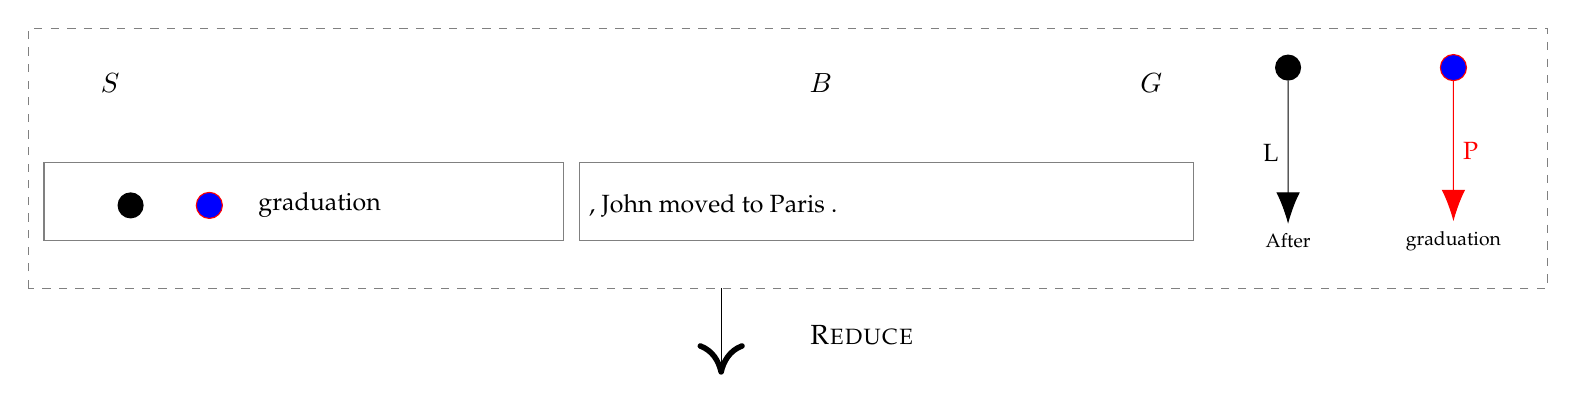
\begin{tikzpicture}[level distance=22mm, sibling distance=4cm]
	\draw[color=gray,dashed] (.2,-.6) rectangle (19.5,2.7);
	\draw[color=gray] (.4,0) rectangle (7,1);
	\node[anchor=west] at (1,2) {$S$};
	\node[fill=black, circle] at (1.5,.45) {};
	\node[fill=blue, draw=red, circle] at (2.5,.45) {};
	\node[anchor=west] at (3,.45) {\small graduation};
	\draw[color=gray] (7.2,0) rectangle (15,1);
	\node[anchor=west] at (10,2) {$B$};
	\node[anchor=west] at (7.2,.45) {\small , John moved to Paris .};
	\node[anchor=west] at (14.2,2) {$G$};
	\node[fill=black, circle] at (16.2,2.2) {}
	  child {node  {\scriptsize After} edge from parent [-{Latex[length=4mm]}] node[left] {\small L}};
	\node[fill=blue, draw=red, circle] at (18.3,2.2) {}
	  child {node {\scriptsize graduation} edge from parent [-{Latex[length=4mm]},red] node[right] {\small P}};
	\node[anchor=west] at (10,-1.2) {\textsc{Reduce}};
	\draw[arrows={->[line width=2pt,length=4mm,width=6mm]}] (9,-.6) -- (9,-1.7);
	\end{tikzpicture}
\end{minipage}
\begin{minipage}{.4\columnwidth}
	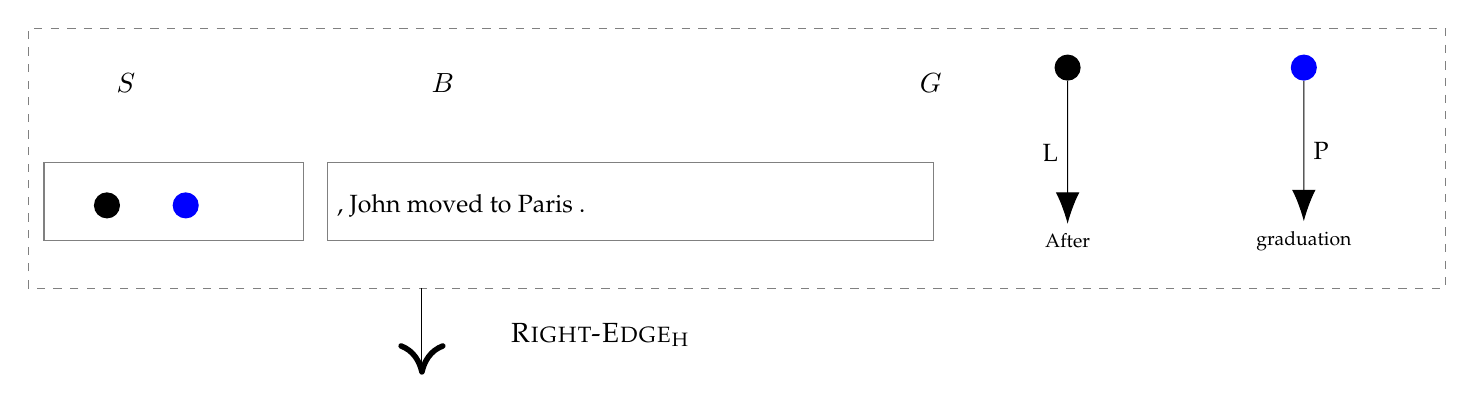
\begin{tikzpicture}[level distance=22mm, sibling distance=4cm]
	\draw[color=gray,dashed] (0,-.6) rectangle (18,2.7);
	\draw[color=gray] (0.2,0) rectangle (3.5,1);
	\node[anchor=west] at (1,2) {$S$};
	\node[fill=black, circle] at (1,.45) {};
	\node[fill=blue, circle] at (2,.45) {};
	\draw[color=gray] (3.8,0) rectangle (11.5,1);
	\node[anchor=west] at (5,2) {$B$};
	\node[anchor=west] at (3.8,.45) {\small , John moved to Paris .};
	\node[anchor=west] at (11.2,2) {$G$};
	\node[fill=black, circle] at (13.2,2.2) {}
	  child {node  {\scriptsize After} edge from parent [-{Latex[length=4mm]}] node[left] {\small L}};
	\node[fill=blue, circle] at (16.2,2.2) {}
	  child {node {\scriptsize graduation} edge from parent [-{Latex[length=4mm]}] node[right] {\small P}};
	\node[anchor=west] at (6,-1.2) {\textsc{Right-Edge\textsubscript H}};
	\draw[arrows={->[line width=2pt,length=4mm,width=6mm]}] (5,-.6) -- (5,-1.7);
	\end{tikzpicture}
	\begin{tikzpicture}[level distance=22mm, sibling distance=4cm]
	\draw[color=gray,dashed] (0,-3.2) rectangle (18,2.7);
	\draw[color=gray] (0.2,0) rectangle (3.5,1);
	\node[anchor=west] at (1,2) {$S$};
	\node[fill=black, circle] at (1,.45) {};
	\node[fill=blue, circle] at (2,.45) {};
	\draw[color=gray] (3.8,0) rectangle (11.5,1);
	\node[anchor=west] at (5,2) {$B$};
	\node[anchor=west] at (3.8,.45) {\small , John moved to Paris .};
	\node[anchor=west] at (12,2) {$G$};
	\node[fill=black, circle] at (14.7,1.5) {}
	  child {node  {\scriptsize After} edge from parent [-{Latex[length=4mm]}] node[left] {\small L}}
	  child {node [fill=blue, circle] {}
	  {
	    child {node {\scriptsize graduation} edge from parent [-{Latex[length=4mm]},black] node[right] {\small P}}
	  } edge from parent [-{Latex[length=5mm]},red] node[right] {\small H} };
	\node[anchor=west] at (6,-3.6) {\textsc{Shift}};
	\draw[arrows={->[line width=2pt,length=4mm,width=6mm]}] (5,-3.2) -- (5,-4.3);
	\end{tikzpicture}
	\begin{tikzpicture}[level distance=22mm, sibling distance=4cm]
	\draw[color=gray,dashed] (0,-3.2) rectangle (18,2.7);
	\draw[color=gray] (0.2,0) rectangle (3.6,1);
	\node[anchor=west] at (1,2) {$S$};
	\node[fill=black, circle] at (1,.45) {};
	\node[fill=blue, circle] at (2,.45) {};
	\node[color=red, anchor=west] at (3,.25) {\small ,};
	\draw[color=gray] (3.9,0) rectangle (11.5,1);
	\node[anchor=west] at (5,2) {$B$};
	\node[anchor=west] at (3.9,.45) {\small John moved to Paris .};
	\node[anchor=west] at (12,2) {$G$};
	\node[fill=black, circle] at (14.7,1.5) {}
	  child {node  {\scriptsize After} edge from parent [-{Latex[length=4mm]}] node[left] {\small L}}
	  child {node [fill=blue, circle] {}
	  {
	    child {node {\scriptsize graduation} edge from parent [-{Latex[length=4mm]}] node[right] {\small P}}
	  } edge from parent [-{Latex[length=5mm]}] node[right] {\small H} };
	\node[anchor=west] at (6,-3.9) {\Large \ldots};
	\draw[arrows={->[line width=2pt,length=4mm,width=6mm]}] (5,-3.2) -- (5,-4.3);
	\end{tikzpicture}
	\begin{tikzpicture}[level distance=22mm, sibling distance=3cm]
	\draw[color=gray,dashed] (0,-5.5) rectangle (18,2.7);
	\draw[color=gray] (.2,0) rectangle (.9,1);
	\node[anchor=west] at (0,2) {$S$};
	\draw[color=gray] (1.3,0) rectangle (2.1,1);
	\node[anchor=west] at (1,2) {$B$};
	\node[anchor=west] at (3,2) {$G$};
    \node (ROOT) [fill=black,circle] at (8,1.5) {}
      child {node (After) {\scriptsize After} edge from parent node[left] {\small L}}
      child {node (graduation) [fill=blue,circle] {}
      {
        child {node {\scriptsize graduation} edge from parent node[left] {\small P}}
      } edge from parent node[left] {\small H} }
      child {node {\scriptsize ,} edge from parent node[right] {\small U}}
      child {node (moved) [fill=purple,circle] {}
      {
        child {node (John) {\scriptsize John} edge from parent node[left] {\small A}}
        child {node {\scriptsize moved} edge from parent node[left] {\small P}}
        child {node [fill=orange,circle] {}
        {
          child {node {\scriptsize to} edge from parent node[left] {\small R}}
          child {node {\scriptsize Paris} edge from parent node[right] {\small C}}
        } edge from parent node[right] {\small A} }
      } edge from parent node[right] {\small H} }
      ;
    \draw[dashed,-{Latex[length=5mm]}] (graduation) to node [auto] {\small A} (John);
	\end{tikzpicture}
\end{minipage}
\captionof{figure}{Example for intermediate states during transition-based parsing.}

Transition-based parsers work by applying a \textit{transition}
at each step to the parser state,
defined using a buffer $B$ of tokens and nodes to be processed,
a stack $S$ of nodes currently being processed,
and a graph $G=(V,E,\ell)$ of constructed nodes and edges.

\vspace{5mm}
A classifier selects the next transition based on the current state's features.
It is trained by an oracle based on gold-standard annotations.
We experiment with three classifiers:
\begin{flushleft}
	\begin{tabular}{ll}
	\textbf{\parser{Sparse}} & Perceptron with features: words, POS, dependency \& edge label combinations. \\
	\textbf{\parser{Dense}} & Perceptron with embedding features: word2vec \cite{mikolov2013efficient} for words, else random. \\
	\textbf{\parser{MLP}} & 2-layer NN, learned embedding features. \\
	\textbf{\parser{BiLSTM}} & 2-layer bidirectional RNN to encode features, 2-layer NN for classification. \\
	\end{tabular}
\end{flushleft}
\vspace{5mm}
For all classifiers, inference is performed greedily, i.e., without beam search.




\section*{Experimental Setup}

\begin{wraptable}{r}{18cm}
	\vspace{-2cm}
	\begin{tabular}{l|ccc|c}
		& \multicolumn{3}{c|}{Wiki} & 20K \\
		& \small Train & \small Dev & \small Test & Leagues \\
		\hline
		\# passages & 300 & 34 & 33 & 154 \\
		\# sentences & 4268 & 454 & 503 & 506 \\
		\hline
		\# nodes & 298,993 & 33,704 & 35,718 & 29,315 \\
		\% terminal & 42.96 & 43.54 & 42.87 & 42.09 \\
		\% non-term. & 58.33 & 57.60 & 58.35 & 60.01 \\
		\% discont. & 0.54 & 0.53 & 0.44 & 0.81 \\
		\% reentrant & 2.38 & 1.88 & 2.15 & 2.03 \\
		\hline
		\# edges & 287,914 & 32,460 & 34,336 & 27,749 \\
		\% primary & 98.25 & 98.75 & 98.74 & 97.73 \\
		\% remote & 1.75 & 1.25 & 1.26 & 2.27 \\
		\hline
		\multicolumn{3}{l}{\footnotesize Average per non-terminal node} \\
		\# children & 1.67 & 1.68 & 1.66 & 1.61 
	\end{tabular}
	\captionof{table}{Statistics of the \textit{Wiki} and \textit{20K Leagues} UCCA corpora.}
\end{wraptable}

Corpora: English Wikipedia, and as
out-of-domain corpus, English part of \textit{Twenty Thousand Leagues Under the Sea}
English-French parallel corpus.

\paragraph{Evaluation.}
Labeled precision, recall and F-score on graph edges, where an edge is represented
by its terminal yield.
Two variants:
\begin{itemize}
\item Primary edges
\item Remote edges
\end{itemize}

\paragraph{Baselines.}

\begin{wrapfigure}{r}{14cm}
	\centering
	\scalebox{.7}{
	\begin{dependency}[theme = simple]
	\begin{deptext}[column sep=.7em,ampersand replacement=\^]
	After \^ graduation \^ , \^ John \^ moved \^ to \^ Paris \\
	\end{deptext}
	\depedge{2}{1}{L}
	\depedge{2}{3}{U}
	\depedge[dashed]{2}{4}{A}
	\depedge{5}{4}{A}
	\depedge{2}{5}{H}
	\depedge{7}{6}{R}
	\depedge{5}{7}{A}
	\end{dependency}
	}
	\scalebox{.7}{
	\begin{dependency}[theme = simple]
	\begin{deptext}[column sep=.7em,ampersand replacement=\^]
	John \^ gave \^ everything \^ up \\
	\end{deptext}
	\depedge{1}{2}{A}
	\depedge{3}{2}{A}
	\depedge{4}{2}{C}
	\end{dependency}
	}
	\scalebox{.7}{
	\begin{dependency}[theme = simple]
	\begin{deptext}[column sep=.7em,ampersand replacement=\^]
	John \^ and \^ Mary \^ went \^ home \\
	\end{deptext}
	\depedge[edge start x offset=-6pt]{1}{4}{A}
	\depedge{2}{1}{N}
	\depedge{3}{1}{C}
	\depedge{5}{4}{A}
	\end{dependency}
	}
	\captionof{figure}{Bilexical approximation for UCCA graphs.}
\end{wrapfigure}

Since there are no existing UCCA parsers, we use bilexical DAG parsers:
\begin{enumerate}
 \item Convert UCCA into bilexical dependencies.
 \item Train parsers on the resulting training set.
 \item Apply trained parsers to the test set.
 \item Reconstruct UCCA graphs.
 \item Compare with gold standard.
\end{enumerate}
Upper bounds are computed by applying
the conversion both ways to the gold standard
graphs and comparing to the original.



\section*{Results}

\parser{BiLSTM} obtains the highest scores in all metrics:
	  
\begin{center}
	\begin{tabular}{l|ccc|ccc||ccc|ccc}
	& \multicolumn{6}{c||}{Wiki (in-domain)} & \multicolumn{6}{c}{20K Leagues (out-of-domain)} \\
	& \multicolumn{3}{c|}{Primary} & \multicolumn{3}{c||}{Remote}
	& \multicolumn{3}{c|}{Primary} & \multicolumn{3}{c}{Remote} \\
	& \textbf{LP} & \textbf{LR} & \textbf{LF} & \textbf{LP} & \textbf{LR} & \textbf{LF}
	& \textbf{LP} & \textbf{LR} & \textbf{LF} & \textbf{LP} & \textbf{LR} & \textbf{LF} \\
	\hline
	\multicolumn{4}{l}{\rule{0pt}{2ex} \footnotesize Bilexical Approximation} \\
	\small Upper Bound
	& \small 94.5 & \small 87.7 & \small 91 & \small 77.3 & \small 46.8 & \small 58.3
	& \small 94.8 & \small 88 & \small 91.3 & \small 66.3 & \small 32.3 & 43.4 \\
	DAGParser \cite{ribeyre-villemontedelaclergerie-seddah:2014:SemEval}
	& 61.8 & 55.8 & 58.6 & 9.5 & 0.5 & 1
	& 56.4 & 50.6 & 53.4 & -- & 0 & 0 \\
	TurboParser \cite{almeida-martins:2015:SemEval}
	& 57.7 & 46 & 51.2 & 77.8 & 1.8 & 3.7
	& 50.3 & 37.7 & 43.1 & 100 & 0.4 & 0.8 \\
	\hline
	\multicolumn{4}{l}{\rule{0pt}{2ex} \footnotesize Direct Approach} \\
	\parser{Sparse}
	& 63.6 & 62.9 & 63.3 & 20.6 & 13.7 & 16.5
	& 59.7 & 59.6 & 59.7 & 26.3 & 8.3 & 12.6 \\
	\parser{Dense} 
	& 59.1 & 58.9 & 59 & 17.4 & 12.4 & 14.5
	& 57.0 & 57.9 & 57.4 & 10.8 & 4.2 & 6.0 \\
	\parser{MLP}
	&  \\
	\parser{BiLSTM}
	&
	\end{tabular}
\end{center}

\begin{wraptable}[7]{l}{15cm}
\hspace{22mm}
\begin{tabular}{l|ccc}
\hline
\multicolumn{4}{l}{\rule{0pt}{2ex} \footnotesize Tree Approximation} \\
\textsc{uparse} \cite{maier-lichte:2016:DiscoNLP} & 60.9 & 61.2 & 6 \\
\hline
\multicolumn{4}{l}{\rule{0pt}{2ex} \footnotesize Bilexical Tree Approximation} \\
\small Upper Bound & \small 94.5 & \small 87.7 & \small 91 \\
MaltParser \cite{nivre2007maltparser} & 62.8 & 57.7 & 60.2 \\
LSTM Parser \cite{dyer2015transition} & 73.2 & 66.9 & 69.9
\end{tabular}
\end{wraptable}

The performance is encouraging in light of
UCCA's inter-annotator agreement of 80--85\%
F-score on primary edges \cite{abend2013universal}.



\paragraph{Tree approximation.}

For completeness, we also explore lossily converting UCCA into trees,
resulting in a simplified task for the underlying parser,
in addition to the maturity of tree-based parsers.

Although remote edges are of pivotal importance, exploring tree approximation methods
can inform the future development of DAG parsers in general and of UCCA parsers in particular.


\section*{Conclusions}

We present \parser{}, the first parser for UCCA, and
evaluate it in both in-domain and out-of-domain settings,
showing it surpasses bilexical DAG parsers on the task of UCCA parsing.

Future work will incorporate LSTMs into \parser{},
and apply the parser to more languages such as German,
demonstrating the importance of broad-coverage parsing.
We will also improve the conversion-based methods and explore different target representations.
A UCCA parser will enable using the scheme for representation in NLP tasks.


\color{DarkSlateGray} % Set the color back to DarkSlateGray for the rest of the content
\tiny
%\nocite{*} % Print all references regardless of whether they were cited in the poster or not
\bibliographystyle{plain} % Plain referencing style
\bibliography{references}

\end{multicols}
\end{document}
